\documentclass[12pt]{article}
\usepackage[paper=letterpaper,margin=1.5cm]{geometry}
\usepackage{amsmath}
\usepackage{amssymb}
\usepackage{amsfonts}
\usepackage{mathtools}
%\usepackage[utf8]{inputenc}
%\usepackage{newtxtext, newtxmath}
\usepackage{lmodern}     % set math font to Latin modern math
\usepackage[T1]{fontenc}
\renewcommand\rmdefault{ptm}
%\usepackage{enumitem}
\usepackage[shortlabels]{enumitem}
\usepackage{titling}
\usepackage{graphicx}
\usepackage[colorlinks=true]{hyperref}
\usepackage{setspace}
\usepackage{subfigure} 
\usepackage{braket}
\usepackage{color}
\usepackage{tabularx}
\usepackage[table]{xcolor}
\usepackage{listings}
\usepackage{mathrsfs}
\usepackage{stackengine}
\usepackage{physics}
\usepackage{afterpage}
\usepackage{pdfpages}
\usepackage[export]{adjustbox}
\usepackage{biblatex}

\setstackEOL{\\}

\definecolor{dkgreen}{rgb}{0,0.6,0}
\definecolor{gray}{rgb}{0.5,0.5,0.5}
\definecolor{mauve}{rgb}{0.58,0,0.82}


\lstset{frame=tb,
  language=Python,
  aboveskip=3mm,
  belowskip=3mm,
  showstringspaces=false,
  columns=flexible,
  basicstyle={\small\ttfamily},
  numbers=none,
  numberstyle=\tiny\color{gray},
  keywordstyle=\color{blue},
  commentstyle=\color{dkgreen},
  stringstyle=\color{mauve},
  breaklines=true,
  breakatwhitespace=true,
  tabsize=3
}
\setlength{\droptitle}{-6em}

\makeatletter
% we use \prefix@<level> only if it is defined
\renewcommand{\@seccntformat}[1]{%
  \ifcsname prefix@#1\endcsname
    \csname prefix@#1\endcsname
  \else
    \csname the#1\endcsname\quad
  \fi}
% define \prefix@section
\newcommand\prefix@section{}
\newcommand{\prefix@subsection}{}
\newcommand{\prefix@subsubsection}{}
\renewcommand{\thesubsection}{\arabic{subsection}}
\makeatother
\DeclareMathOperator*{\argmin}{argmin}
\newcommand{\partbreak}{\begin{center}\rule{17.5cm}{2pt}\end{center}}
\newcommand{\alignbreak}{\begin{center}\rule{15cm}{1pt}\end{center}}
\newcommand{\tightalignbreak}{\vspace{-5mm}\alignbreak\vspace{-5mm}}
\newcommand{\hop}{\vspace{1mm}}
\newcommand{\jump}{\vspace{5mm}}
\newcommand{\R}{\mathbb{R}}
\newcommand{\C}{\mathbb{C}}
\newcommand{\N}{\mathbb{N}}
\newcommand{\G}{\mathbb{G}}
\renewcommand{\S}{\mathbb{S}}
\newcommand{\bt}{\textbf}
\newcommand{\xdot}{\dot{x}}
\renewcommand{\star}{^{*}}
\newcommand{\ydot}{\dot{y}}
\newcommand{\lm}{\mathrm{\lambda}}
\renewcommand{\th}{\theta}
\newcommand{\id}{\mathbb{I}}
\newcommand{\si}{\Sigma}
\newcommand{\Si}{\si}
\newcommand{\inv}{^{-1}}
\newcommand{\T}{^\intercal}
\renewcommand{\tr}{\text{tr}}
\newcommand{\ep}{\varepsilon}
\newcommand{\ph}{\varphi}
%\renewcomand{\norm}[1]{\left\lVert#1\right\rVert}
\definecolor{cit}{rgb}{0.05,0.2,0.45}
\addtolength{\jot}{1em}
\newcommand{\solution}[1]{

\noindent{\color{cit}\textbf{Solution:} #1}}

\newcounter{tmpctr}
\newcommand\fancyRoman[1]{%
  \setcounter{tmpctr}{#1}%
  \setbox0=\hbox{\kern0.3pt\textsf{\Roman{tmpctr}}}%
  \setstackgap{S}{-.9pt}%
  \Shortstack{\rule{\dimexpr\wd0+.1ex}{.9pt}\\\copy0\\
              \rule{\dimexpr\wd0+.1ex}{.9pt}}%
}

\newcommand{\Id}{\fancyRoman{2}}

% Enter the specific assignment number and topic of that assignment below, and replace "Your Name" with your actual name.
\title{STAT 31050: Homework 1}
\author{Caleb Derrickson}
\date{April 1, 2024}

\begin{document}
\onehalfspacing
\maketitle
\allowdisplaybreaks

\tableofcontents

\newcommand{\barP}{\Bar{P}}
\newcommand{\barQ}{\Bar{Q}}
\renewcommand{\braket}[2]{\langle #1, #2 \rangle}

\newpage
\section{Exercise 1}
Prove that the Trapezoid rule follows the following error inequality for integration:
\[|T_n(f) - I(f)| \leq \frac{C}{n^2}\norm{f''}_\infty.\]
\partbreak
\begin{solution}

    The overview of my solution will be first showing the error for $n = 1$ for generic bounds $(a, b)$, then applying that to the case for $n \neq 1$ (I will explain this better when we get to it). For $n = 1$, and assuming our function $f$ is at least twice differentiable, then by Taylor's Theorem, \footnote{I am citing the Wikipedia page for Taylor's Theorem.} 
    \[f(x) = f(a) + f'(a)(x - a) + R_1(x).\]
    Here, the term $R_1(x)$ represents the remainder term, in particular the mean value form of it. This is given as 
    \[R_1(x) = \frac{f''(\xi_L)}{2}(x - a)^2,\]
    where $a \leq \xi_L \leq b$. Since the point we are expanding from in Taylor's Theorem is generic ( within $[a, b]$), we can also expand from the point $x = b$ to get 
    \[f(x) = f(b) + f'(b)(x - b) + R_1(x).\]
    The remainder term is slightly different in this case, where we have\footnote{The value $\xi_L$ is somewhat loose here; I am assuming it is equal over different Taylor expansions, since the remainder term, or the Peano remainder term at least, is unique. This does not change the calculation, since we would just sum over the sup norm at the end.} 
    \[R_1(x) = \frac{f''(\xi_L)}{2}(x - a)^2.\]
    Since these two expansions are equivalent, we can sum them both and divide to get the original function, so
    \[f(x) = \frac{1}{2}(f(a) + f(b)) + \frac{1}{2}\left[f'(a)(x - a) +f'(b)(x - b)\right] + \frac{f''(\xi_L)}{4}[(x - a)^2 + (x - b)^2]\]
    Integrating from $a$ to $b$, and after some factorization, we get 
    \begin{align*}
        \int_a^b f(x) \ dx &= \frac{1}{2}(f(a) + f(b)) + \frac{1}{2}f'(a) \left( \frac{1}{2}(b - a)^2\right) + \frac{1}{2}f'(b) \left( -\frac{1}{2}(b - a)^2\right) + \frac{f''(\xi_L)}{6}(b-a)^3\\
        &= \frac{1}{2}(f(a) + f(b))+ \frac{(b - a)^2}{4}[f'(a) - f'(b)] + \frac{f''(\xi_L)}{6}(b - a)^3.
    \end{align*}
    Since $f \in C^2([a, b])$, for some $\eta \in [a, b]$, we can apply the Mean Value Theorem to the first term to get
    \[\int_a^b f(x) \ dx = \frac{1}{2}(f(a) + f(b)) - \frac{f''(\eta)}{4}(b - a)^3 + \frac{f''(\xi_L)}{6}(b - a)^3,\]
    note the minus sign, which comes from inverting the Mean Value Theorem. Comparing with the first term of Trapezoid integration, 
    \[T_1(f) = \frac{f(a) + f(b)}{2},\]
    we see that this is the first term in integration. To get the error in Trapezoid integration, we then have
    \[E_1 = |I(f) - T_1(f)| = (b - a)^3\left|\frac{f''(\eta)}{4} - \frac{f''(\xi_L)}{6}\right|,\]
    where I assume $a < b$. Since $f''$ is continuous, there exists a value, which I will denote as $m$, which attains the maximum value for $f''$ on the interval $[a, b]$. We then have
    \[E_1 = |I(f) - T_1(f)| \leq  \frac{(b - a)^3}{12}|f''(m)| = \frac{(b - a)^3}{12}\norm{f''}_\infty.\]
    
    Therefore, the first order Trapezoid error is bounded by the above result. When we go to the case where $n \neq 1$, that is, when we consider summing over any number of trapezoid approximations, we can apply this error to each interval $[x_{j-1}, x_j]$ in question. That is, if we consider partitioning the interval $[0, 1]$ into intervals $[x_{j-1}, x_j]$ and approximating the function $f(x)$ over that interval by the Trapezoid method, then we can apply the error term for each interval, and sum over them. This is what I take as "gluing," which is mentioned in the hint. \par

    \jump
    Since the function $f$ is continuous, we can then split up the integral with respect to the above mentioned partition. Note that I have not mentioned the explicit form of the $x_i$ terms - we will take them to be evenly spaced between $[0, 1]$ by the formula $x_j = jh$, where $j \in \N$ with $j \leq n$ and $h = \frac{1}{n}$. We then have 
    \[I(f) \leadsto \sum_{j = 1}^n \int_{x_{j-1}}^{x_j} f(x) \ dx.\]
    On each interval $[x_{j-1}, x_j]$, we approximate the function by a trapezoid, which will incur error by the above result. Setting bounds $a = x_{j-1}$ and $b = x_j$, we have the individual error terms as 
    \[E([x_{j-1}, x_j]) = \frac{h^3}{12}\norm{f''}_{\infty, j}, \quad x_{j-1} \leq c_j \leq x_j.\]

    Note the sup norm is over the specific interval rather than the total interval. The total error in integration is then summing over all $j$, which will give us 
    \[E_n(f) = \frac{h^3}{12}\sum_{j = 1}^n \norm{f''}_{\infty, j}.\]

    The max value attained on each interval is certainly smaller than the maximum value over the total interval, so we can bound the error by swapping the sup values. Noticing that the sum is independent of $j$, we get that 
    \[E_n(f) \leq \frac{nh^3}{12}\norm{f''}_{\infty} = \frac{1}{12n^2}\norm{f''}_{\infty},\]

    which, when setting $M = \frac{1}{12}$, we get the desired form. 
    
\end{solution}

\newpage
\section{Exercise 3}
Assuming that $f \in C^4(0, 1)$, construct an improved quadrature rule which computes the integral of $f$ on $(0, 1)$ with an error which is $O(\frac{1}{n^4})$. Your rule should only involve a constant number of modifications to the standard left-hand or right-hand Riemann sums as $n \into \infty$. Implement your quadrature rule and plot the convergence for:
\begin{itemize}
    \item $f(x) = e^x$
    \item $f(x) = \sqrt{x}$
\end{itemize}
Compare your numerical results with those obtained from Simpson’s rule – using a cubic approximation on each subinterval, where the cubic is chosen to agree with f at the two endpoints and the midpoint of each subinterval.

\newpage
\section{Exercise 4}
Let $\{v_j\}_{j = 1}^\infty$ be an orthonormal basis of a Hilbert space $\scH$. Let $A$ be a bounded operator from $\scH$ to itself, with bounded inverse. Consider the sequence of vectors $w_j := Av_j$. Is $\{w_j\}_{j = 1}^\infty$ an orthonormal basis? A Schauder basis? If so, can you bound its basis constant?

\newcommand{\scX}{\mathcal{X}}

\newpage
\section{Exercise 5}
Let $\psi : \R \to \R$ be the function defined by 
\[\psi(x) = \begin{cases}
    0, &x \not \in (0, 1),\\
    2x, &x \in [0, 1/2],\\
    2(1 - x), &x \in [1/2, 1].
\end{cases}\]
For $i = 0, ..., \infty$ and $k = 0, ..., 2^i - 1$ define $\psi_{i, k}$ by 
\[\psi_{i, k}(x) = \psi(2^ix + k)\]
Consider the collection of functions $\scX = \{1, x, \psi_{0, 0}, \psi_{1, 0}, \psi_{1, 1}, \psi_{2, 0}, ...\}$. Sketch the first five functions of $\scX$ on $[0, 1]$. Show that $\scX$ is a Schauder basis of $C([0, 1])$. 
\partbreak
\begin{solution}

    I do not like adding hand-written sketches in homework, since I find them to be too messy for any meaningful interpretation. Instead, I have included a plot of the first five functions of $\scX$ in Figure \ref{fig:Exercise5} using Python. We will next show that $\scX$ is a Schauder basis of $C([0, 1])$. That is, we need to show that there exists unique coefficients $\alpha_1, \alpha_2, ...$ for which
    \[v = \sum_{j = 1}^\infty \alpha_j \scX_j \quad \text{for all } v \in C([0, 1]).\]
    Note that $C([0, 1])$ equipped with the sup-norm is a Banach space, since the space of continuous functions on a compact interval (the interval $[0, 1]$ is closed and bounded) is a Banach Space. This tells us that the problem is well posed. This problem is in essence an existence and uniqueness exercise; we will first show existence. 
\end{solution}

\newpage
\vspace{5in}
\begin{figure}
    \centering
    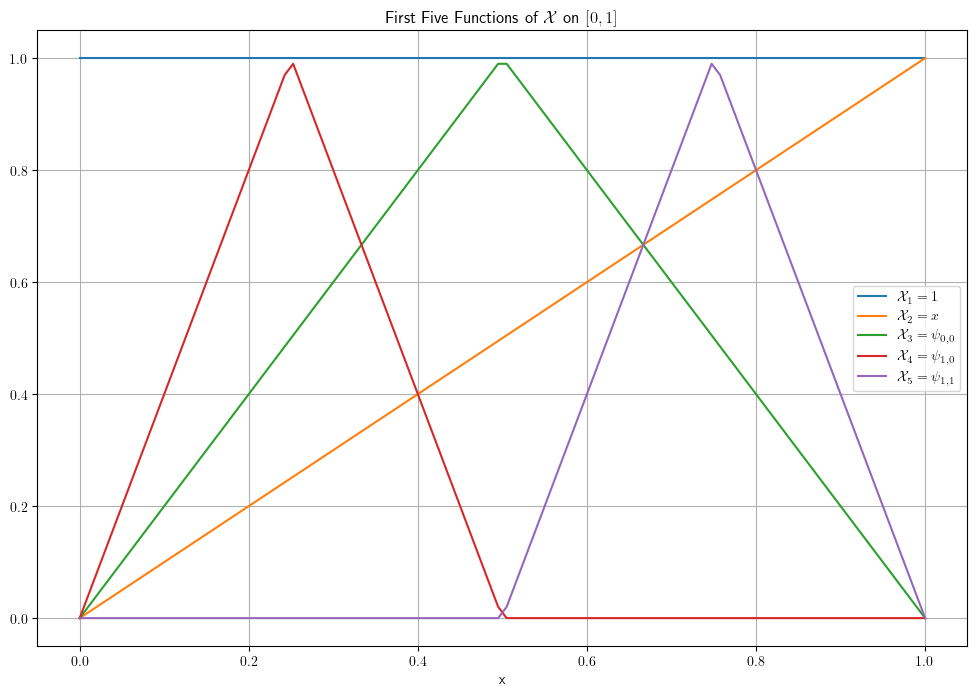
\includegraphics[width = 0.8\textwidth]{Figures/Exercise5.png}
    \caption{First five functions of $\scX$ for Exercise 5.}
    \label{fig:Exercise5}
\end{figure}
\clearpage

\newpage
\section{Exercise 6}
Let $\scH$ be a Hilbert space and let $P, Q: \scH \to \scH$ be two projections. In the following, set $C = i[P, Q] = i(PQ - QP)$. We also assume that $P$ and $Q$ are orthogonal, $i.e.$ $P\star = P$ and $Q\star = Q$.
\subsection{Exercise 6, part a}
Find explicit examples of $P$ and $Q$ which do not commute. Make sure to give clear definitions of both them and $\scH$. Sketch a geometric characterization of when this happens. 

\newpage
\subsection{Exercise 6, part b}
Show that $0 \leq \braket{v}{Pv} \leq 1$ for all $v \in \scH$. 

\newpage
\subsection{Exercise 6, part c}
For any $v \in \scH$, set $\barP(v) = \braket{v}{Pv}, \barQ(v) = \braket{v}{Qv}, \sigma^2_P(v) = \braket{v}{(P - \barP \id)^2}$ and $\sigma_Q^2 = \braket{v}{(Q - \barQ \id)^2 v}$. Show that $\sigma_P, \sigma_Q \leq \norm{v} / 2$. Here, $\id$ is the identity operator on $\scH$.  

\newpage
\subsection{Exercise 6, part d}
If $C$ is the commuatator of $P$ and $Q$, show that $\frac{1}{4}|\braket{v}{Cv}|^2 \leq \sigma_P^2(v) \sigma_Q^2(v).$ Argue that $\norm{C} \leq 1/2$. For the last part, you can use without proof that $\norm{C} = \sup_{\norm{v}\leq 1} |\braket{v}{Cv}|$ (this follows from the fact that $C$ is Hermitian).
\end{document}